\documentclass[a4paper, 11pt]{report}
\usepackage{graphicx}
\usepackage{subcaption}
\begin{document}

\section{parallel computing}
	\subsection{What is parallel computing}
The problem when facing large calculations is that they require a lot of computing power and time. Performing these calculations can be done in different types of computation but the most common ones are serial and parallel computation. Serial computing means, you have one compute unit (e.g. a single core CPU) available to deal with all the calculations that have to be done on a certain set of data. The problem will be broken into multiple smaller subproblems that will be solved by a certain instruction. The single compute unit has to perform the instruction on every subproblem to solve the main problem as shown in figure \ref{fig:SerialC}.
	\begin{figure}[h]
		\centering
		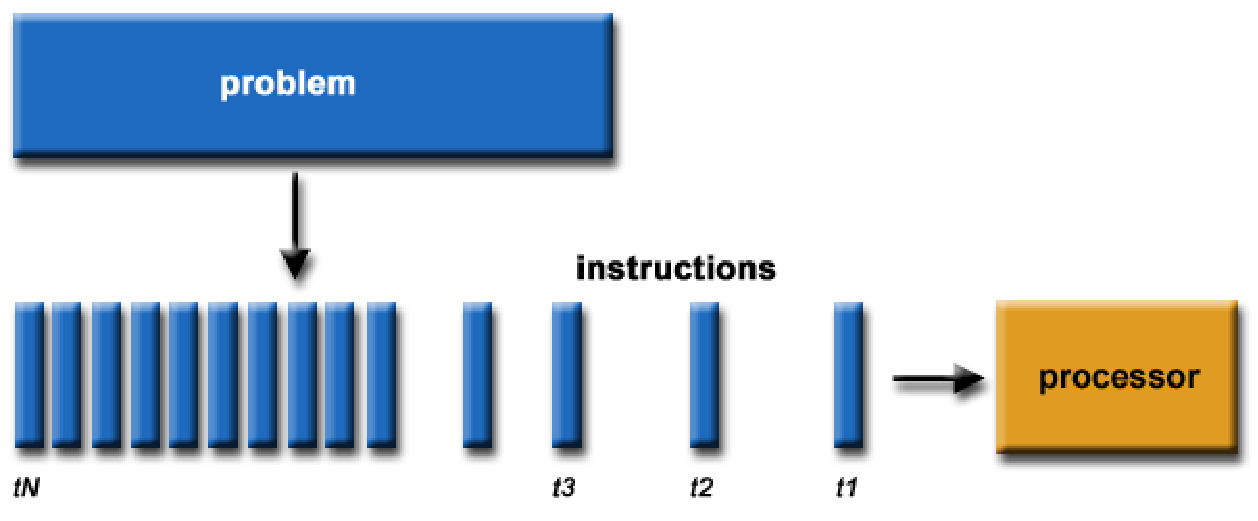
\includegraphics[scale=.4]{images/serialProblem.pdf}
		\caption{Workflow serial computing}
		\label{fig:SerialC}
	\end{figure}\\
Parallel computing, on the other hand, is the simultaneous use of multiple compute units (CPU+GPU), or a compute resource, to solve a computational problem. We break apart the main problem in smaller subproblems as we did with serial computing. Each part is further broken down to a series of instructions again.Now, since there are multiple compute units, we can distribute the subproblems among all these compute units. Every unit can now perform the instruction on their given subproblems simultaneously as shown in figure \ref{fig:ParallelC}. One compute resource can constist of multiple compute units, for example it can include multiple processors or it's just a number of computers connected by a network.
	\begin{figure}[h]
		\centering
		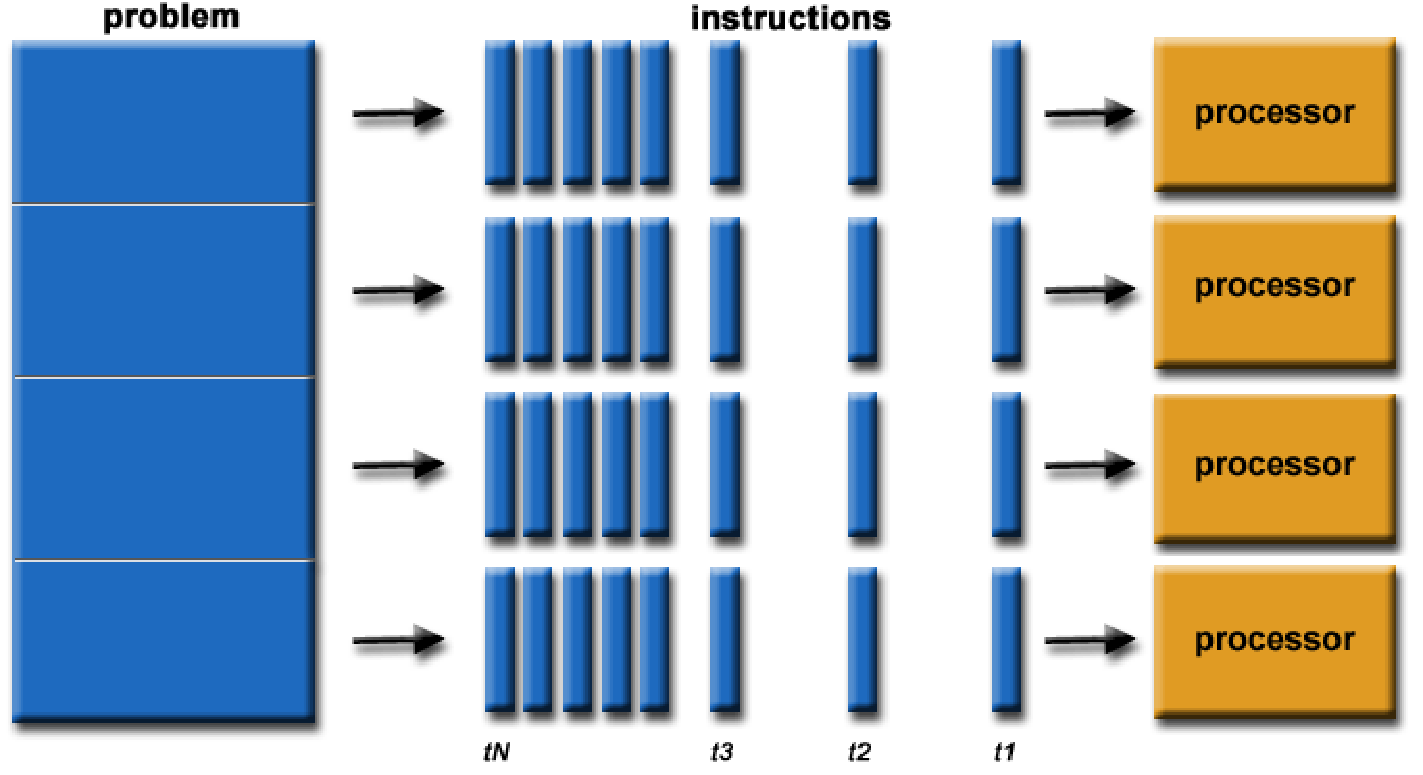
\includegraphics[scale=.4]{images/parallelProblem.pdf}
		\caption{Workflow parallel computing}
		\label{fig:ParallelC}
	\end{figure}\\
With multiple compute units for one task, we will shorten the completion time aswell have potential cost savings. It also allows us to solve larger/complex problems since a single computer could suffer from limited memory. And last, we are able to access non-local resources in a network that wouldn't be accessable from a local computer.\\ It is easy to conclude that the concept of parallel computing was to have a more efficient way to handle with large sets of data such as images or simulations that involve multiple parameters. It's also easier to handle with complex data for example in algorithms.

	\subsection{Classification of parallel computing}
Parallel computing systems can be seperated into different classes. According to Flynn's taxonomy we can roughly place any of these systems in one of the four classes he defined. The classifications are determined by two factors: instruction stream and data stream which both have two possible states being single or multiple. Figure \ref{fig:flynnTaxonomy} represents a matrix of the four possible classes from the Flynn's taxonomy.

	\begin{figure}[h]
		\centering
		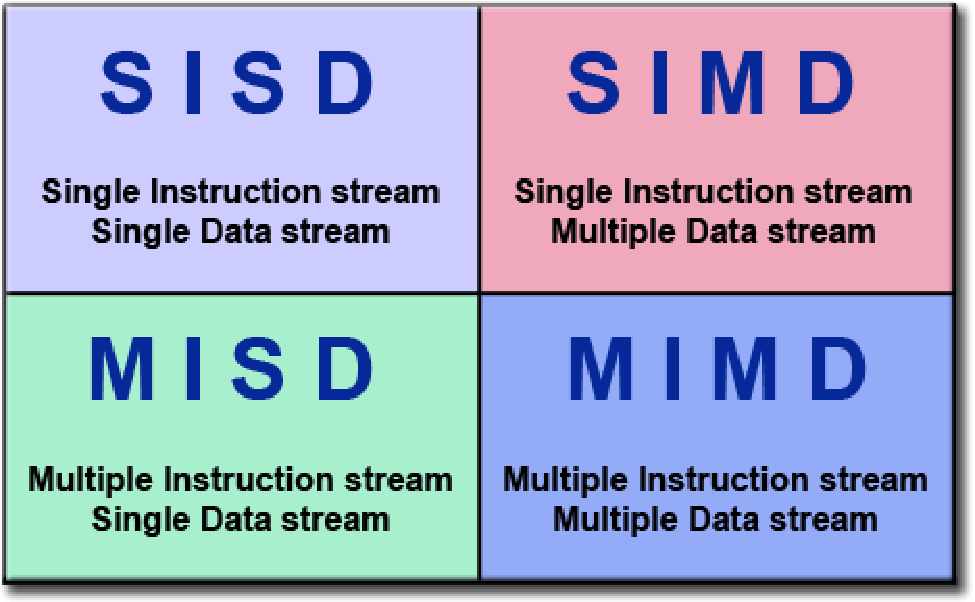
\includegraphics[scale=.5]{images/flynnsTaxonomy.pdf}
		\caption{Four possible classifications according to Flynn's Taxonomy}
		\label{fig:flynnTaxonomy}
	\end{figure}
	
	\begin{itemize}
		\item SISD
	\end{itemize}
The SISD class will have a single processor executing a single data stream to operate on data stored in a single memory (figure \ref{fig:sisd}). This means that a parallel compute system cannot be classified as an SISD sytem, but Flynn's taxonomy wasn't made for just classifying parallel compute systems. It's usually old computers and other older compute units that can be classified as SISD.
	\begin{itemize}
		\item SIMD
	\end{itemize}
Data is disctributed amongst multiple processors who all execute the same instruction (figure \ref{fig:simd}). Since we have access to multiple compute units, parallel computing can be categorized in this class. Furthermore, this is the class where we can categorize our subject of the thesis in since we have a large set of data divided over multiple data streams (MD) and only one instruction stream (SI) since all processing units will perform the same instruction on the data. The SIMD class contains most modern computers, particularly those with a graphics processor unit (GPU).

	\begin{itemize}
		\item MISD
	\end{itemize}
Each processing unit operates on the data independently via separate instruction streams
	
	\begin{itemize}
		\item MIMD
	\end{itemize}

\begin{figure*}[h]
	\centering
	\begin{subfigure}[t]{0.4\textwidth}
		\centering
		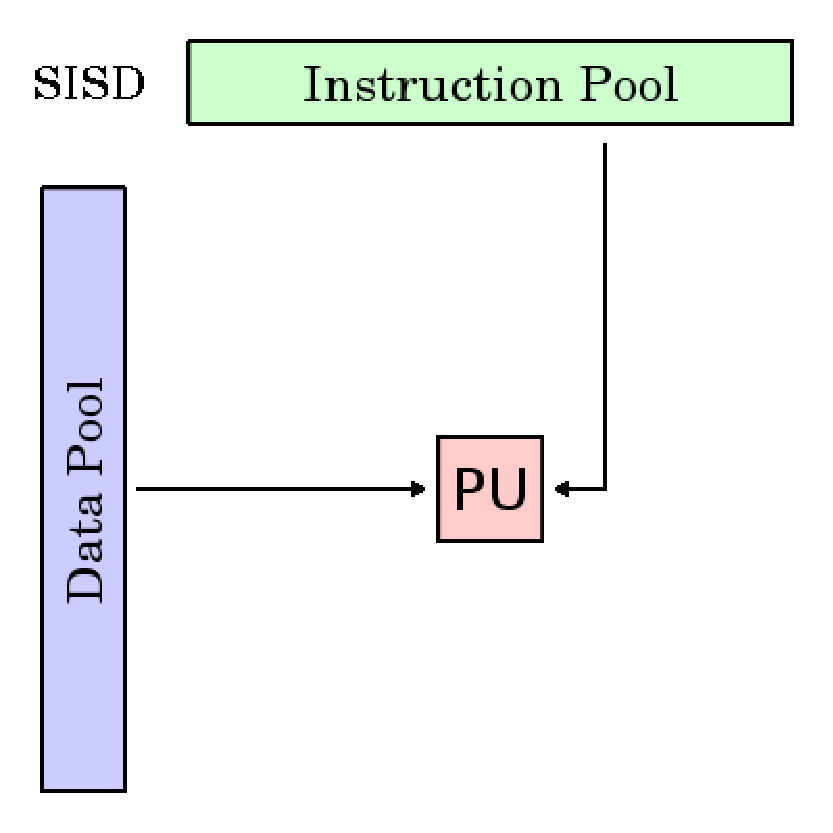
\includegraphics[scale=.3]{images/sisd.pdf}
		\caption{SISD}\label{fig:sisd}
	\end{subfigure}
	\begin{subfigure}[t]{0.4\textwidth}
		\centering
		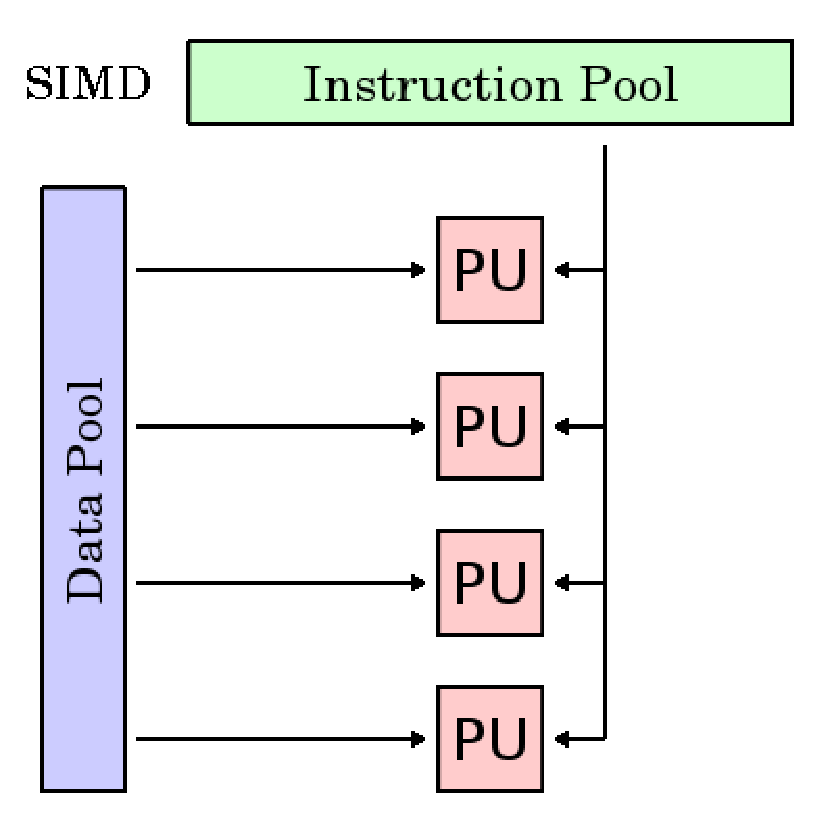
\includegraphics[scale=.3]{images/simd.pdf}
		\caption{SIMD}\label{fig:simd}
	\end{subfigure}
	\begin{subfigure}[t]{0.4\textwidth}
		\centering
		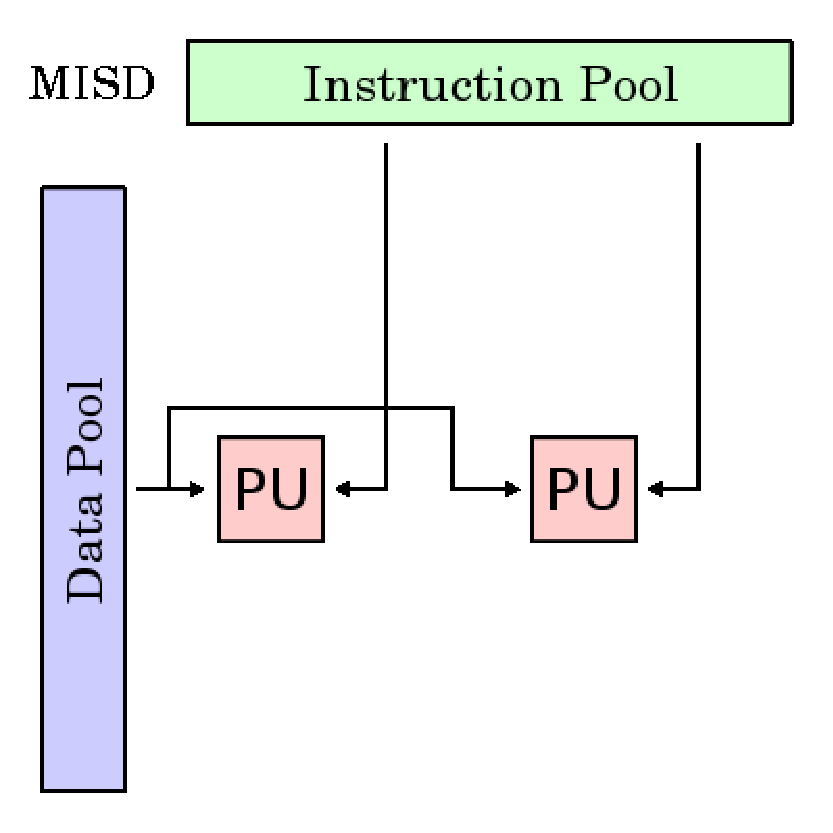
\includegraphics[scale=.3]{images/misd.pdf}
		\caption{MISD}\label{fig:misd}
	\end{subfigure}
	\begin{subfigure}[t]{0.4\textwidth}
		\centering
		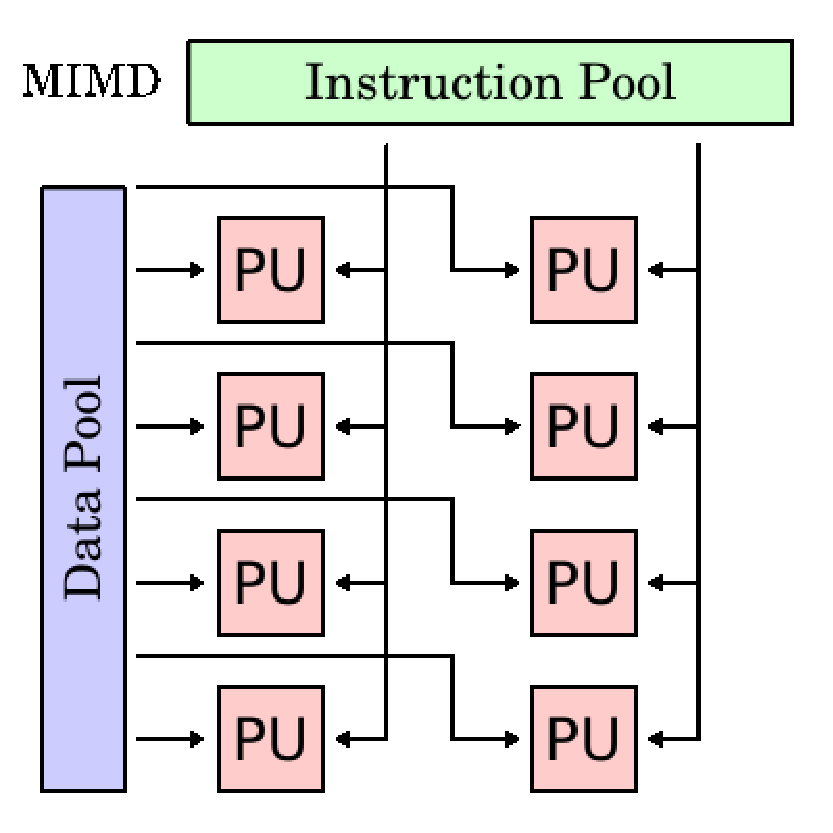
\includegraphics[scale=.3]{images/mimd.pdf}
		\caption{MIMD}\label{fig:mimd}
	\end{subfigure}
	\caption{Architecture classes from Flynn's taxonomy}\label{fig:archFlynnTax}
		
		
	
\end{figure*}

	\subsection{Amdahl's law and Gustafson's law}
		\begin{itemize}
			\item Amdahl's Law
		\end{itemize}
Amdahl's Law 

	\subsection{OpenCL}\label{subsec:OpenCL}




\bibliographystyle{IEEEtran}
\bibliography{References}
\end{document}
